%%%%%%%%%%%%%%%%%%%%%%%%%%%%%%%%%%%%%%%%%
% Structured General Purpose Assignment
% LaTeX Template
%
% This template has been downloaded from:
% http://www.latextemplates.com
%
% Original author:
% Ted Pavlic (http://www.tedpavlic.com)
%
% Note:
% The \lipsum[#] commands throughout this template generate dummy text
% to fill the template out. These commands should all be removed when 
% writing assignment content.
%
%%%%%%%%%%%%%%%%%%%%%%%%%%%%%%%%%%%%%%%%%

%----------------------------------------------------------------------------------------
%	PACKAGES AND OTHER DOCUMENT CONFIGURATIONS
%----------------------------------------------------------------------------------------

\documentclass{article}

\usepackage{fancyhdr} % Required for custom headers
\usepackage{lastpage} % Required to determine the last page for the footer
\usepackage{extramarks} % Required for headers and footers
\usepackage{graphicx} % Required to insert images
\usepackage{lipsum} % Used for inserting dummy 'Lorem ipsum' text into the template
\usepackage{listings}
\usepackage{color}
\usepackage{amsmath}

\definecolor{dkgreen}{rgb}{0,0.6,0}
\definecolor{gray}{rgb}{0.5,0.5,0.5}
\definecolor{mauve}{rgb}{0.58,0,0.82}

\lstset{frame=tb,
  language=R,
  aboveskip=3mm,
  belowskip=3mm,
  showstringspaces=false,
  columns=flexible,
  basicstyle={\small\ttfamily},
  numbers=none,
  numberstyle=\tiny\color{gray},
  keywordstyle=\color{blue},
  commentstyle=\color{dkgreen},
  stringstyle=\color{mauve},
  breaklines=true,
  breakatwhitespace=true
  tabsize=3
}

% Margins
\topmargin=-0.45in
\evensidemargin=0in
\oddsidemargin=0in
\textwidth=6.5in
\textheight=9.0in
\headsep=0.25in 

\linespread{1.1} % Line spacing

% Set up the header and footer
\pagestyle{fancy}
\lhead{\hmwkAuthorName} % Top left header
\chead{\hmwkClass\ (\hmwkClassInstructor\ \hmwkClassTime): \hmwkTitle} % Top center header
\rhead{\firstxmark} % Top right header
\lfoot{\lastxmark} % Bottom left footer
\cfoot{} % Bottom center footer
\rfoot{Page\ \thepage\ of\ \pageref{LastPage}} % Bottom right footer
\renewcommand\headrulewidth{0.4pt} % Size of the header rule
\renewcommand\footrulewidth{0.4pt} % Size of the footer rule

\setlength\parindent{0pt} % Removes all indentation from paragraphs

%----------------------------------------------------------------------------------------
%	DOCUMENT STRUCTURE COMMANDS
%	Skip this unless you know what you're doing
%----------------------------------------------------------------------------------------

% Header and footer for when a page split occurs within a problem environment
\newcommand{\enterProblemHeader}[1]{
\nobreak\extramarks{#1}{#1 continued on next page\ldots}\nobreak
\nobreak\extramarks{#1 (continued)}{#1 continued on next page\ldots}\nobreak
}

% Header and footer for when a page split occurs between problem environments
\newcommand{\exitProblemHeader}[1]{
\nobreak\extramarks{#1 (continued)}{#1 continued on next page\ldots}\nobreak
\nobreak\extramarks{#1}{}\nobreak
}

\setcounter{secnumdepth}{0} % Removes default section numbers
\newcounter{homeworkProblemCounter} % Creates a counter to keep track of the number of problems

\newcommand{\homeworkProblemName}{}
\newenvironment{homeworkProblem}[1][Problem \arabic{homeworkProblemCounter}]{ % Makes a new environment called homeworkProblem which takes 1 argument (custom name) but the default is "Problem #"
\stepcounter{homeworkProblemCounter} % Increase counter for number of problems
\renewcommand{\homeworkProblemName}{#1} % Assign \homeworkProblemName the name of the problem
\section{\homeworkProblemName} % Make a section in the document with the custom problem count
\enterProblemHeader{\homeworkProblemName} % Header and footer within the environment
}{
\exitProblemHeader{\homeworkProblemName} % Header and footer after the environment
}

\newcommand{\problemAnswer}[1]{ % Defines the problem answer command with the content as the only argument
\noindent\framebox[\columnwidth][c]{\begin{minipage}{0.98\columnwidth}#1\end{minipage}} % Makes the box around the problem answer and puts the content inside
}

\newcommand{\homeworkSectionName}{}
\newenvironment{homeworkSection}[1]{ % New environment for sections within homework problems, takes 1 argument - the name of the section
\renewcommand{\homeworkSectionName}{#1} % Assign \homeworkSectionName to the name of the section from the environment argument
\subsection{\homeworkSectionName} % Make a subsection with the custom name of the subsection
\enterProblemHeader{\homeworkProblemName\ [\homeworkSectionName]} % Header and footer within the environment
}{
\enterProblemHeader{\homeworkProblemName} % Header and footer after the environment
}
   
%----------------------------------------------------------------------------------------
%	NAME AND CLASS SECTION
%----------------------------------------------------------------------------------------

\newcommand{\hmwkTitle}{Homework 1} % Assignment title
\newcommand{\hmwkDueDate}{Aug 5,\ 2014} % Due date
\newcommand{\hmwkClass}{Statistics} % Course/class
\newcommand{\hmwkClassTime}{6:00 pm} % Class/lecture time
\newcommand{\hmwkClassInstructor}{Instructor: Rados Radoicic} % Teacher/lecturer
\newcommand{\hmwkAuthorName}{Weiyi Chen} % Your name

%----------------------------------------------------------------------------------------
%	TITLE PAGE
%----------------------------------------------------------------------------------------

\title{
\vspace{2in}
\textmd{\textbf{\hmwkClass:\ \hmwkTitle}}\\
\normalsize\vspace{0.1in}\small{Due\ on\ \hmwkDueDate}\\
\vspace{0.1in}\large{\textit{\hmwkClassInstructor\ \hmwkClassTime}}
\vspace{3in}
}

\author{\textbf{\hmwkAuthorName}}
\date{} % Insert date here if you want it to appear below your name

%----------------------------------------------------------------------------------------

\begin{document}

\maketitle

%----------------------------------------------------------------------------------------
%	TABLE OF CONTENTS
%----------------------------------------------------------------------------------------

%\setcounter{tocdepth}{1} % Uncomment this line if you don't want subsections listed in the ToC

%\newpage
%\tableofcontents
\newpage

%----------------------------------------------------------------------------------------
%	PROBLEM 1
%----------------------------------------------------------------------------------------

\begin{homeworkProblem}
    \begin{homeworkSection}{The standard Student's t distribution}
        The standard Student's t distribution is a special case of Student's t distribution. By first explaining this special case, the exposition of the more general case is greatly facilitated. The standard Student's t distribution is characterized as follows: \\
        \textbf{Definition:} We say that $X$ has a standard Student's t distribution with $n$ degrees of freedom if its probability density function is:
        \begin{equation}
            f_X(x) = c(1+\frac{x^2}{n})^{-(n+1)/2}
        \end{equation}
        where $c$ is a constant:
        \begin{equation}
            c = \frac{1}{\sqrt{n}} \frac{1}{B(\frac{n}{2},\frac{1}{2})}
        \end{equation}
        where $B()$ is a beta function. \\
        \textbf{Proposition:} The probability density function of $X$ can be written as:e
        \begin{equation}
            f_X(x) = \int_0^\infty f_{X|Z=z}(x)f_Z(z)dz
        \end{equation}
        where $f_{X|Z=z}(x)$ is the probability density function of a normal distribution with mean 0 and variance $\sigma^2 = \frac{1}{2}$, $f_Z(z)$ is the probability density function of a Gamma random variable with parameters $n$ and $h=1$. This is obvious. If $X$ is a zero-mean normal random variable with variance $1/z$, conditional on $Z=z$, then we can think of $X$ as a ratio:
        \begin{equation}
            X = \frac{Y}{\sqrt{Z}}
        \end{equation}
        where $Y$ has a standard normal distribution, $Z$ has a Gamma distribution and $Y$ and $Z$ are independent. \\
        \textbf{Expected value:} The expected value of a standard Student's t random variable  X is well-defined only for $n>1$ and it is equal to:
        \begin{equation}
            E[X] = 0
        \end{equation}
        It follows from the fact that the density function is symmetric around $0$:
        \begin{equation}
            \begin{split}
                E[X] &= \int_{-\infty}^0xf_X(x)dx + \int_{0}^{\infty}xf_X(x)dx \\
                &= -\int_{0}^{\infty}xf_X(x)dx + \int_{0}^{\infty}xf_X(x)dx \\
                &= 0
            \end{split}
        \end{equation}
        by exchanging the bounds of integraton and $f_X(x) = f_X(x)$. The above integrals are finite (and so the expected value is well-defined) only if $n>1$, because
        \begin{equation}
            \begin{split}
                \int_0^{\infty} &= \lim_{u \to \infty} \int_0^u xc(1+\frac{x^2}{n})^{-(n+1)/2} dx \\
                &= c \int_0^u \left[-\frac{n}{n-1}(1+\frac{x^2}{n})^{-(n-1)/2}\right]_0^u \\
                &= \frac{-cn}{n-1} \left[\lim_{u\to\infty}(1+\frac{u^2}{n})^{-\frac{1}{2}(n-1)} \right]
            \end{split}
        \end{equation}
        and the above limit is finite only if $n>1$. \\
        \textbf{Variance:} The variance of a standard Student's t random variable $X$ is well-defined only for $n>2$ and it is equal to:
        \begin{equation}
            Var[X] = \frac{n}{n-2}
        \end{equation}
        It can be derived thanks to the usual variance formula ($Var(X) = E[X^2] - (E[X])^2$) and to the integral representation of the Beta function:
        \begin{equation}
            \begin{split}
                E[X^2] &= \int_{-\infty}^{\infty} x^2 f_X(x) dx \\
                &= 2 \int_0^{\infty} x^2 f_X(x) dx \\
                &= 2c \int_0^{\infty} x^2 (1+\frac{x^2}{n})^{-(n+1)/2} dx \\
                &= 2c \int_0^{\infty} n(1+t)^{-n/2-1/2} \frac{\sqrt{n}}{2} \frac{1}{\sqrt{t}}dt \\
                &= cn^{3/2} \int_0^{\infty} t^{3/2-1} (1+t)^{-3/2-(n/2-1)}dt \\
                &= cn^{3/2} B(\frac{3}{2}, \frac{n}{2}-1) \\
                &= \frac{1}{\sqrt{n}} \frac{1}{B(\frac{n}{2},\frac{1}{2})} n^{3/2} B(\frac{3}{2}, \frac{n}{2}-1) \\
                &= n \frac{\Gamma(n/2+1/2)}{\Gamma(n/2)\Gamma(1/2)} \frac{\Gamma(1/2+1)\Gamma(n/2-1)}{n/2+1/2} \\
                &= n \frac{\Gamma(1/2)\frac{1}{2}\Gamma(n/2)\frac{2}{n-2}}{\Gamma(1/2)\Gamma(n/2)} \\
                &= \frac{n}{n-2}
            \end{split}
        \end{equation}
        Therefore using $(E[X])^2 = 0$,
        \begin{equation}
            Var[X] = E[X^2] - (E[X])^2 = \frac{n}{n-2}
        \end{equation}
        From the above derivation, it should be clear that the variance is well-defined only when $n>2$. Otherwise, if $n \leq 2$, the above improper integrals do not converge (and the Beta function is not well-defined).
    \end{homeworkSection}
    \begin{homeworkSection}{Student's t distribution in general}
        \textbf{Definition:} We say that $X$ has a Student's t distribution with mean $\mu$, scale $\sigma^2$ and $n$ degrees of freedom if its probability density function is:
        \begin{equation}
            f_X(x) = \frac{c}{\sigma} (1+\frac{(x-\mu)^2}{n\sigma^2})^{-\frac{n+1}{2}}
        \end{equation}
        where $c$ is a constant:
        \begin{equation}
            c = \frac{1}{\sqrt{n}B(n/2,1/2)} 
        \end{equation}
        and $B() $ is the Beta function. A random variable $X$ which has a t distribution with mean $\mu$, scale $\sigma^2$ and $n$ degrees of freedom is just a linear function of a standard Student's t random variable:
        \begin{equation}
            X = \mu + \sigma Z
        \end{equation}
        where $Z$ is a random variable having a standard t distribution. \\
        \textbf{Expectation:} The expected value of a Student's t random variable $X$ is well-defined only for $n>1$ and it is equal to:
        \begin{equation}
            E[X] = \mu
        \end{equation}
        It is an immediate consequence of the fact that $X=\mu+\sigma Z$ and the linearity of the expected value:
        \begin{equation}
            E[X] = E[\mu + \sigma Z] = \mu + \sigma E[Z] = \mu + \sigma 0 = \mu
        \end{equation}
        As we have seen above, $E[Z]$ is well-defined only for $n>1$ and, as a consequence, also $E[X]$ is well-defined only for $n>1$. \\
        \textbf{Variance:} The variance of a Student's t random variable $X$ is well-defined only for $n>2$ and it is equal to:
        \begin{equation}
            Var[X] = \frac{n}{n-2} \sigma^2
        \end{equation}
        It can be derived using the formula for the variance of affine transformations on $X=\mu +\sigma Z$:
        \begin{equation}
            Var[X] = Var[\mu + \sigma Z] = \sigma^2 Var[Z] = \sigma^2 \frac{n}{n-2}
        \end{equation}
        As we have seen above, $Var[Z]$ is well-defined only for $n>2$ and, as a consequence, also $Var[X]$ is well-defined only for $n>2$.
    \end{homeworkSection}
\end{homeworkProblem}

%----------------------------------------------------------------------------------------
%   PROBLEM 2
%----------------------------------------------------------------------------------------

\begin{homeworkProblem}
    \begin{homeworkSection}{Gamma mgf}
        The gamma pdf is given
        \begin{equation}
            f(x) = \frac{1}{\Gamma(\alpha)\beta^\alpha} x^{\alpha-1}e^{-x/\beta}
        \end{equation}
        for $0 < x < \infty, \alpha > 0, \beta>0$, where $\Gamma(\alpha)=\int_0^\infty t^{\alpha-1}e^{-t}dt$ denotes the gamma function. The mgf is
        \begin{equation}
            \begin{split}
                M_X(t) &= \frac{1}{\Gamma(\alpha)\beta^\alpha} \int_0^\infty e^{tx}x^{\alpha-1}e^{-x/\beta} \\
                &= \frac{1}{\Gamma(\alpha)\beta^\alpha} \int_0^\infty x^{\alpha-1}e^{-x/(\frac{\beta}{1-\beta t})} \\
                &= \frac{1}{\Gamma(\alpha)\beta^\alpha} \Gamma(\alpha) (\frac{\beta}{1-\beta t})^{\alpha} \\
                &= (\frac{1}{1-\beta t})^\alpha
            \end{split}     
        \end{equation} 
        for $t < \frac{1}{\beta}$. If $t \ge \frac{1}{\beta}$ then the quantity $1-\beta t$ is nonpositive and the integral is infinite. Thus, the mgf of the gamma distribution exists only if $t < 1/\beta$. \\
    \end{homeworkSection}
    \begin{homeworkSection}{Gamma skewness and kurtosis}
        Gamma mgf giving the logarithmic moment-generating function as
        \begin{equation}
            \begin{split}
                \mu_0 &= R(t) = -\alpha \ln(1-\beta t) \\
                \mu_1 &= R'(t) = \frac{\alpha \beta}{1-\beta t} \\
                \mu_2 &= R''(t) = \frac{\alpha \beta^2}{(1-\beta t)^2} \\
                \mu_3 &= R^{(3)}(t) = \frac{2\alpha \beta^3}{(1-\beta t)^3} \\
                \mu_4 &= R^{(4)}(t) = \frac{6\alpha \beta^4}{(1-\beta t)^4}
            \end{split}
        \end{equation}
        The skewness and kurtosis are then
        \begin{equation}
            \begin{split}
                \gamma_1 &= \frac{\mu_3}{\mu_2^{3/2}} = \frac{2}{\sqrt{\alpha}} \\
                \gamma_2 &= \frac{\mu_4}{\mu_2^2} = \frac{6}{\alpha} + 3
            \end{split}
        \end{equation}
    \end{homeworkSection}
\end{homeworkProblem}

%----------------------------------------------------------------------------------------
%   PROBLEM 3
%----------------------------------------------------------------------------------------

\begin{homeworkProblem}
    \begin{homeworkSection}{(a)}
        We have two Normal distributions $N_1 \sim N(0,1)$ and $N_2 \sim N(0, 10)$ with the same mean (which without loss of generality is set to zero) but with different standard deviations. we form a mixture, $M$, of these two different distributions, i.e. a distribution where the probability of drawing from the first distribution is $p_1 = 95\%$ and from the second distribution is $p_2 = 5\%$. The kurtosis of the mixture is as follows:
        \begin{equation}
            \frac{3(p_1\sigma_1^4+p_2\sigma_2^4)}{(p_1\sigma_1^2+p_2\sigma_2^2)^2} - 3 = \frac{3(0.95\times1+0.05\times100)}{(0.95\times1+0.05\times10)^2} -3 = 5.489893
        \end{equation}
    \end{homeworkSection}
    \begin{homeworkSection}{(b)}
        Actually I have used that formula as a conclusion in my part(a). I will show how to derive it in this part. Let $X_1, ..., X_n$ denote random variables from the $n$ component distributions, and let $X$ denote a random variable from the mixture distribution. Then, for any function $H()$ for which $\operatorname{E}[H(X_i)]$ exists, and assuming that the component densities $p_i(x)$ exist (to distinguish, I use $w$ to denote weights here.)
        \begin{align}
            \operatorname{E}[H(X)] & = \int_{-\infty}^\infty H(x) \sum_{i = 1}^n w_i p_i(x) \, dx \\
            & = \sum_{i = 1}^n w_i \int_{-\infty}^\infty p_i(x) H(x) \, dx = \sum_{i = 1}^n w_i \operatorname{E}[H(X_i)].
        \end{align}
        The relation,
        \begin{equation}
            \operatorname{E}[H(X)] =  \sum_{i = 1}^n w_i \operatorname{E}[H(X_i)],
        \end{equation}
        holds more generally. \\
        It is a trivial matter to note that the jth moment about zero (i.e. choosing $H(x) = x^j$) is simply a weighted average of the jth moments of the components. Moments about the mean $H(x) = (x − \mu)^j$ involve a binomial expansion:
        \begin{align}
            \operatorname{E}[(X - \mu)^j] &= \sum_{i = 1}^n w_i \operatorname{E}[(X_i - \mu_i + \mu_i - \mu)^j] \\
            &= \sum_{i=1}^n \sum_{k=0}^j \left( \begin{array}{c} j \\ k \end{array} \right) (\mu_i - \mu)^{j-k} w_i \operatorname{E}[(X_i- \mu_i)^k],
        \end{align}
        where $\mu_i$ denotes the mean of the ith component. \\
        In case of a mixture of one-dimensional normal distributions with weights $w_i$, means $\mu_i$ and variances $\sigma_i^2$, the total mean and variance will be:
        \begin{align}
             \operatorname{E}[X] &= \mu = \sum_{i = 1}^n w_i \mu_i ,\\
             \operatorname{E}[(X - \mu)^2] &= \sigma^2 = \sum_{i=1}^n w_i((\mu_i - \mu)^{2} + \sigma_i^2) \\
        \end{align}
        Similarly we are able to derive $\operatorname{E}[(X - \mu)^3], \operatorname{E}[(X - \mu)^4]$ and the kurtosis is
        \begin{align}
            \gamma_2 &= \frac{\operatorname{E}[(X - \mu)^4]}{(\operatorname{E}[(X - \mu)^2])^2} - 3 \\
            &= \frac{1}{\sigma^4}\sum_{i=1}^{n}{w_i}[3\sigma_i^4+6(\mu_i-\mu)^2\sigma_i^2+(\mu_i-\mu)^4] - 3
        \end{align}
        In our problem, there are only two components with $p_1 = p, p_2 = 1-p$, $\mu_1 = \mu_2 = 0$, $\sigma_1 = 1, \sigma_2 = \sigma$ as parameters, then
        \begin{equation}
            \gamma_2 = \frac{3[p+(1-p)\sigma^4]}{[p+(1-p)\sigma^2]^2} - 3
        \end{equation}
    \end{homeworkSection}
    \begin{homeworkSection}{(c)}
        We can rewrite $\gamma_2$ as
        \begin{align}
            \gamma_2 &= \frac{3(1-p)\sigma^4+3p}{(1-p)^2\sigma^4 + 2(1-p)p\sigma^2 + p^2} - 3
        \end{align}
        Then we take $\sigma = 1/(1-p)$ (my intuition is to make $p$ very close to 1 and $\sigma$ very large)
        \begin{equation}
            \gamma_2 = \frac{3(1-p)+3p(1-p)^4}{(1-p)^2+2(1-p)^{3}p+p^2(1-p)^4} - 3
        \end{equation}
        When $p \to 1$, or when $q = 1-p \to 0$,
        \begin{equation}
            \lim_{p\to 1}\gamma_2 = \lim_{q\to 0} \frac{3q + 3(1-q)q^4}{q^2 + 2(1-q)q^{3} + (1-q)^2q^4} - 3 = \lim_{q\to 0} \frac{3}{q} - 3 \to \infty
        \end{equation}
        which means kurtosis can be arbitrarily large. \\
        To find values of $\sigma$ and $p$ so that the kurtosis is 10000, we can just let $\sigma = 1/(1-p)$
        \begin{equation}
            \gamma_2 = \frac{3(1-p)+3p(1-p)^4}{(1-p)^2+2(1-p)^{3}p+p^2(1-p)^4} - 3 = 10000
        \end{equation}
        which generates
        \begin{equation}
            p \approx 0.9997, \sigma \approx 3334.3
        \end{equation}
    \end{homeworkSection}
    \begin{homeworkSection}{(d)}
        In this part, our goal is to construct $p$ and $\sigma$, to reach a kurtosis at least $M$. Again we can continue using the same constrution as did in part(c), take $p = p_0 + \epsilon$ ($\epsilon \in (0, 1-p_0)$) and $\sigma = 1/(1-p)$, we still have the kurtosis as
        \begin{equation}
            \gamma_2 = \frac{3(1-p)+3p(1-p)^4}{(1-p)^2+2(1-p)^{3}p+p^2(1-p)^4} - 3
        \end{equation}
        No matter $p_0$ how close to 1, that is $p_0 \to 1$, we also have $p = p_0 + \epsilon \to 1$, then we let
        \begin{equation}
            \lim_{p \to 1}\gamma_2 = 3/(1-p) - 3 \ge M
        \end{equation}
        which generates
        \begin{equation}
            p \ge \frac{M}{M+3}
        \end{equation}
        If we take 
        \begin{equation}
            p = \max\{\frac{M}{M+3}, p_0\}, \sigma = \frac{1}{1-p}
        \end{equation}
        we are able to get a kurtosis at least $M$.
    \end{homeworkSection}
\end{homeworkProblem}

%----------------------------------------------------------------------------------------
%   PROBLEM 4
%----------------------------------------------------------------------------------------

\begin{homeworkProblem}
    \begin{homeworkSection}{(A)}
        For a Poisson distribution,
        \begin{align}
            f(x_1, x_2, \dots, x_n| \lambda) &= \frac{e^{-\lambda}\lambda^{x_1}}{x_1!}\frac{e^{-\lambda}\lambda^{x_2}}{x_2!}\dots\frac{e^{-\lambda}\lambda^{x_n}}{x_n!} = \frac{e^{-n\lambda}\lambda^{\sum x_i}}{x_1!x_2!\dots x_n!} \\
            \ln f &= -n\lambda+(\ln \lambda)\sum x_i - \ln(\prod x_i!) \\
            \frac{d(\ln f)}{d\lambda} &= -n + \frac{\sum x_i}{\lambda} = 0\\
            \hat \lambda &= \frac{\sum x_i}{n}
        \end{align}
        It is easy to verify that
        \begin{equation}
            \frac{\partial^2}{\partial \lambda^2} \log f(x|\lambda) = -\frac{x}{\lambda^2}
        \end{equation}
        Therefore the Fisher information is
        \begin{equation}
            I(\lambda) = -E[-\frac{X}{\lambda^2}] = \frac{1}{\lambda}
        \end{equation}
        The asymptotic normality of MLE is
        \begin{equation}
            \sqrt{n}(\hat \lambda - \lambda_0) \to N(0, \lambda_0) 
        \end{equation}
    \end{homeworkSection}
    \begin{homeworkSection}{(B)}   
        For a normal distribution $N(\mu, \sigma^2)$ where $\sigma^2$ is known. The likelihood function is
        \begin{equation}
            L(x_1, x_2, \dots, x_n| \mu) = (2\pi\sigma^2)^{-n/2} \exp(-\frac{1}{2\sigma^2} \sum_{j=1}^n (x_j-\mu)^2)
        \end{equation}
        The log-likelihood function is
        \begin{equation}
            l(x_1, x_2, \dots, x_n| \mu) = -\frac{n}{2}\ln(2\pi) - \frac{n}{2}\ln(\sigma^2) - \frac{1}{2\sigma^2} \sum_{j=1}^n (x_j - \mu)^2
        \end{equation}
        The partial derivative of the log-likelihood with respect to the mean is
        \begin{equation}
            \frac{\partial}{\partial \mu}l(x_1, x_2, \dots, x_n| \mu) = \frac{1}{\sigma^2} (\sum_{j=1}^n x_j - n\mu) = 0
        \end{equation}
        Therefore the maximum likelihood estimator of the mean is
        \begin{equation}
            \hat \mu = \frac{1}{n} \sum_{j=1}^n x_j
        \end{equation}
        It is easy to verify that
        \begin{equation}
            \frac{\partial^2}{\partial \mu^2}l(x| \mu) = -\frac{1}{\sigma^2}
        \end{equation}
        Therefore the Fisher information is
        \begin{equation}
            I(\mu) = -E[-\frac{1}{\sigma^2}] = \frac{1}{\sigma^2}
        \end{equation}
        The asymptotic normality of MLE is
        \begin{equation}
            \sqrt{n}(\hat \mu - \mu_0) \to N(0, \sigma^2) 
        \end{equation}
    \end{homeworkSection}
    \begin{homeworkSection}{(C)}
        For a normal distribution $N(\mu, \sigma^2)$ where $\mu = 0$ is known. The likelihood function is
        \begin{equation}
            L(x_1, x_2, \dots, x_n| \sigma) = (2\pi\sigma^2)^{-n/2} \exp(-\frac{1}{2\sigma^2} \sum_{j=1}^n x_j^2)
        \end{equation}
        The log-likelihood function is
        \begin{equation}
            l(x_1, x_2, \dots, x_n| \sigma) = -\frac{n}{2}\ln(2\pi) - \frac{n}{2}\ln(\sigma^2) - \frac{1}{2\sigma^2} \sum_{j=1}^n x_j^2
        \end{equation}
        The partial derivative of the log-likelihood with respect to the variance is
        \begin{equation}
            \frac{\partial}{\partial \sigma^2}l(x_1, x_2, \dots, x_n| \sigma) = \frac{1}{2\sigma^2} (\frac{1}{\sigma^2} \sum_{j=1}^n x_j^2 - n)
        \end{equation}
        Therefore the maximum likelihood estimator of the variance is
        \begin{equation}
            \hat\sigma^2 = \frac{1}{n} \sum_{j=1}^n x_j^2
        \end{equation}
        It is easy to verify that
        \begin{equation}
            \frac{\partial^2}{(\partial \sigma^2)^2}l(x| \sigma) = -\frac{x^2}{\sigma^6} + \frac{1}{2\sigma^4}
        \end{equation}
        Therefore the Fisher information is
        \begin{equation}
            I(\sigma^2) = -E[-\frac{X^2}{\sigma^6} + \frac{1}{2\sigma^4}] = \frac{1}{2\sigma^4}
        \end{equation}
        The asymptotic normality of MLE is
        \begin{equation}
            \sqrt{n}(\hat \sigma^2 - \sigma_0^2) \to N(0, 2\sigma_0^4) 
        \end{equation}
    \end{homeworkSection}
\end{homeworkProblem}

%----------------------------------------------------------------------------------------
%   PROBLEM 5
%----------------------------------------------------------------------------------------

\begin{homeworkProblem}
    \begin{homeworkSection}{MLE of $b$}
        Uniform distribution has p.d.f.
        \begin{equation}
            f(x|b) = 
            \begin{cases}
                \frac{1}{b-a}, &a\le b \\
                0, &\text{otherwise}
            \end{cases}
        \end{equation}
        First note that $f(x|b)=1/(b-a)$, for $a\le x\le b$ and $0$ elsewhere. Then it is easy to see that the likelihood function is given by
        \begin{equation}
            L(b|x) = \prod_{i=1}^n \frac{1}{b-a}I(X_i \in [a,b]) = (b-a)^{-n}I(max(X_1,\dots,X_n)\le b)
        \end{equation}
        Here the indicator function $I(A)$ equals to $1$ if event $A$ happens and $0$ otherwise. What the indicator above means is that the likelihood will be equal to $0$ if at least one of the factors is $0$ and this will happen if at least one observation $X_i$ will fall outside of the allowed interval $[a, b]$. Another way to say it is that the maximum among observations will exceed $b$, i.e.
        \begin{equation}
            L(b) = 0 \text{ if } b < \max(X_1, X_2, \dots, X_n)
        \end{equation}
        and
        \begin{equation}
            L(b) = \frac{1}{(b-a)^n} \text{ if } b \ge \max(X_1, X_2, \dots, X_n)
        \end{equation}
        which is a decreasing function in the second part. Therefore $\hat b = \max(X_1, \dots, X_n)$ is the MLE.
    \end{homeworkSection}
    \begin{homeworkSection}{MLE of $a$}
        Follow the same step in the previous part and using the property of symmetry, MLE of $a$ is
        \begin{equation}
            \hat a = \min(X_1, \dots, X_n) 
        \end{equation}
    \end{homeworkSection}
    \begin{homeworkSection}{MLE of mean $\mu$}
        According to the invariance property of MLE, $\hat a$ and $\hat b$ are the MLE of $a$ and $b$, then $g(\hat a, \hat b)$ is the MLE of $g(a, b)$ for any one-to-one function $g$, respectively for $a$ and $b$. So for the mean $\mu$, we will let
        \begin{equation}
            g(a,b) = \frac{a+b}{2}
        \end{equation}
        Therefore, MLE of $\mu$ is
        \begin{equation}
            \hat \mu = g(\hat a, \hat b) = \frac{\hat a + \hat b}{2} = \frac{\max(X_1, X_2, \dots, X_n) + \min(X_1, \dots, X_n)}{2}
        \end{equation}
    \end{homeworkSection}
\end{homeworkProblem}

%----------------------------------------------------------------------------------------
%   PROBLEM 6
%----------------------------------------------------------------------------------------

\begin{homeworkProblem}
    \begin{homeworkSection}{Problem 1}
        \centerline{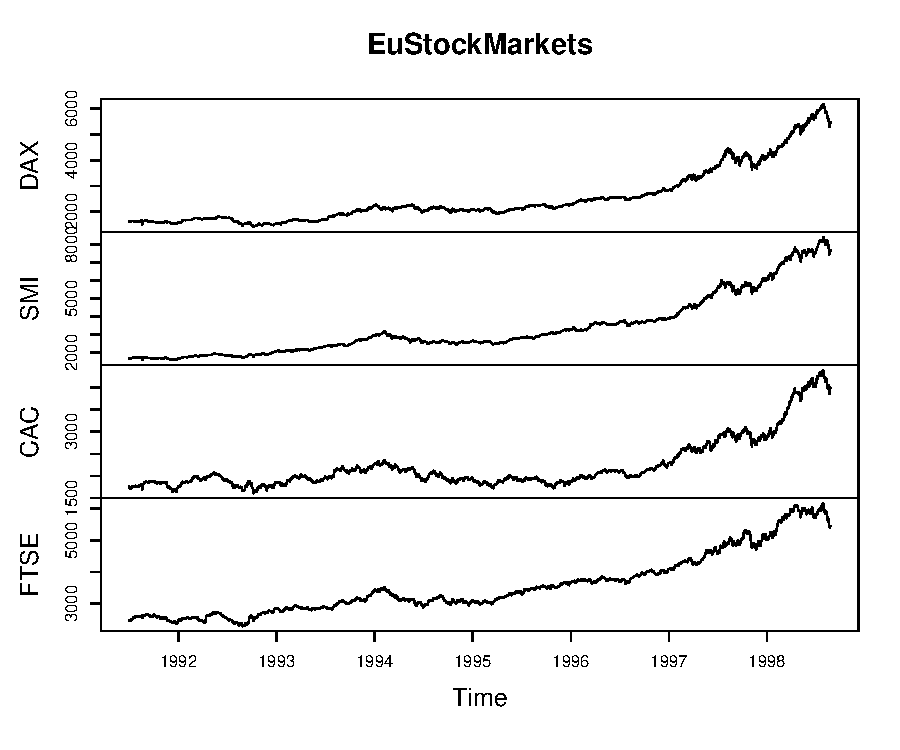
\includegraphics[scale=0.7]{EuStocks.pdf}}
        The series does not look stationary. The fluctuations does not seem to be of constant size, the volatility becomes larger and larger when time passes.
    \end{homeworkSection}
    \begin{homeworkSection}{Problem 2}
        \centerline{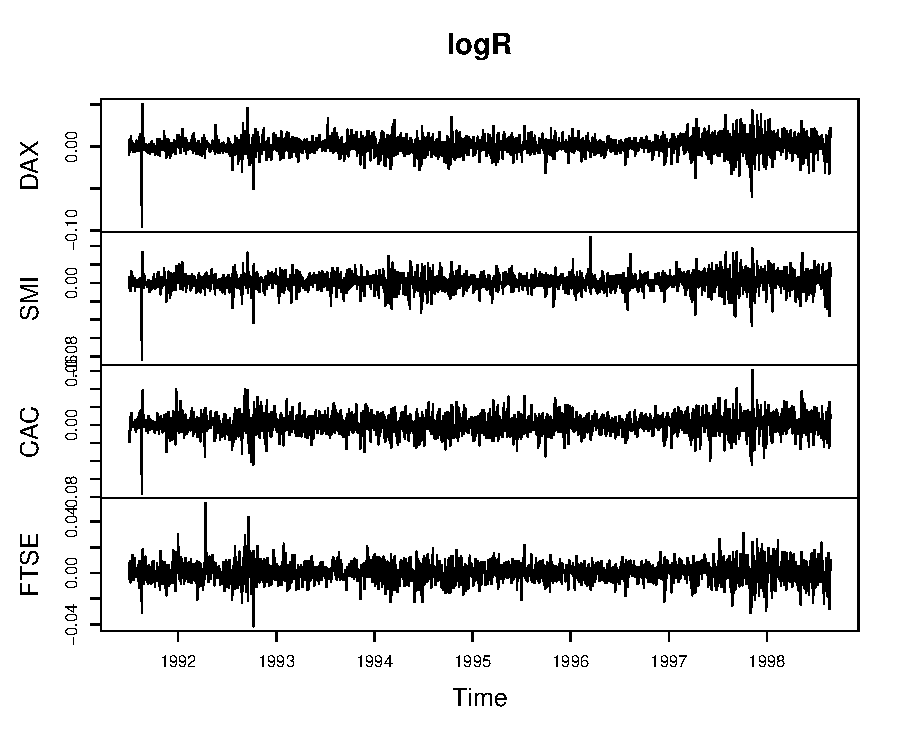
\includegraphics[scale=0.7]{logEuStocks.pdf}}
        The series looks stationary. The fluctuations seems to be of constant size.
    \end{homeworkSection}
    \begin{homeworkSection}{Problem 3}
        \centerline{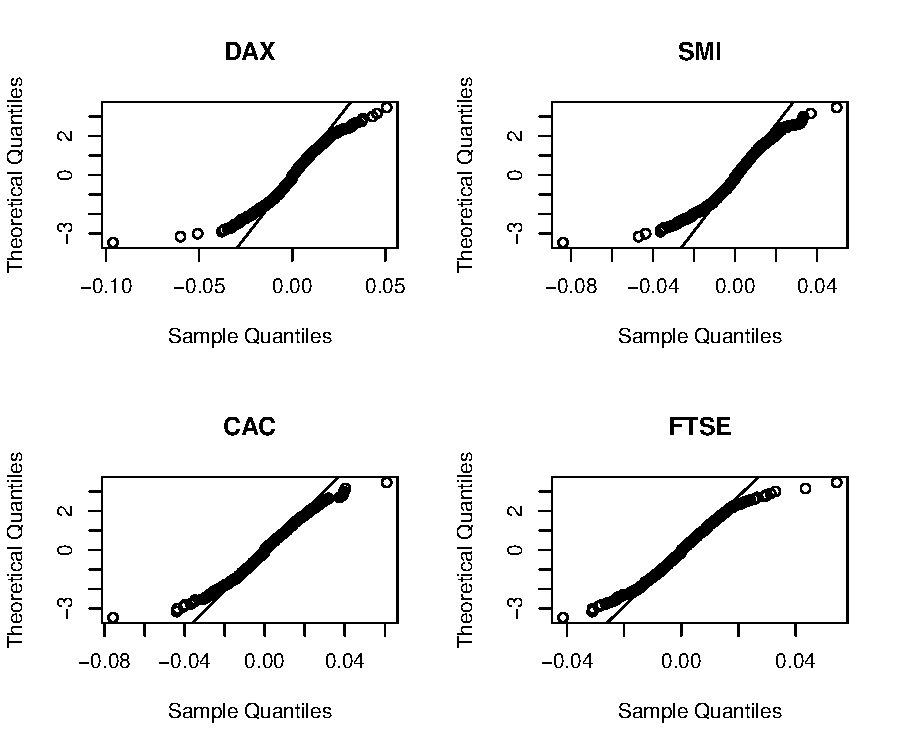
\includegraphics[scale=0.7]{quantile.pdf}}
        The marginal distribution of all series are symmetric and their tails appear heavier than a normal distribution. This is the printed out results
        \begin{lstlisting}
    Shapiro-Wilk normality test

data:  logR[, i]
W = 0.9538, p-value < 2.2e-16


    Shapiro-Wilk normality test

data:  logR[, i]
W = 0.9554, p-value < 2.2e-16


    Shapiro-Wilk normality test

data:  logR[, i]
W = 0.982, p-value = 1.574e-14


    Shapiro-Wilk normality test

data:  logR[, i]
W = 0.9799, p-value = 1.754e-15
        \end{lstlisting}
        All the Shapiro-Wilk tests reject the null hypothesis of normality with extremely small p-values.\\
    \end{homeworkSection}
    I don't have time to accomplish the left tests, sorry. 
\end{homeworkProblem}

\end{document}